\documentclass{beamer}
\usepackage[russian]{babel}
\usetheme{metropolis}

\usepackage{amsthm}
\usepackage{ulem}
\setbeamertemplate{theorems}[numbered]

\setbeamercolor{block title}{use=structure,fg=white,bg=gray!75!black}
\setbeamercolor{block body}{use=structure,fg=black,bg=gray!20!white}

\usepackage[T2A]{fontenc}
\usepackage[utf8]{inputenc}

\usepackage{hyphenat}
\usepackage{amsmath}
\usepackage{graphicx}

\AtBeginEnvironment{proof}{\renewcommand{\qedsymbol}{}}{}{}

\title{
Микроэкономика-I
}
\author{
Павел Андреянов, PhD
}

\begin{document}

\maketitle

\begin{frame}{План лекции}
\begin{itemize}
  \item Часть 1. РВ с функциями издержек, РВ с линейными функциями
  \item Часть 2. Mеждународная торговля.
\end{itemize}
\end{frame}

\section{РВ с функциями издержек}

\begin{frame}{РВ с функциями издержек}
Обычно, когда речь идет о равновесии Вальраса, мы не обговариваем, какие ресурсы являются факторами, а какие потребительскими товарами.

Однако, легко представить ситуацию, в которой полезность агента вообще не зависит от некоторых товаров.

Тогда я мог бы задать поведение фирмы при помощи функции издержек, главное чтобы они были выпуклые по конечному товару и вогнуты по ценам факторов
\end{frame}

\section{Пример 1}

\begin{frame}{Пример 1}
Рассмотрим пример с 2 фирмами и 1 агентом
\begin{gather*}
	U_a(x_1, x_2, x_3) = \log x_2 + \log x_3, \quad w = (1,0,0)\\
	TC_{\alpha}(x_2) = x_2^2 \\
	TC_{\beta}(x_3) = x_3^2 
\end{gather*}
Агент владеет обеими фирмами

Вектор цен нормирован $(1, p, q)$.

Попробуем решить...
\end{frame}

\begin{frame}{Пример 1}
Выпишем прибыли каждой фирмы
\begin{gather*}
	\pi_{\alpha} = p x_2 - x_2^2, \quad 
	\pi_{\beta} = q x_3 - x_3^2
\end{gather*}
Выпишем условия первого порядка
\begin{gather*}
	x^*_{2,\alpha} = p/2, \quad 
	x^*_{3,\beta} = q/2
\end{gather*}
Выпишем прибыли опять
\begin{gather*}
	\pi^*_{\alpha} = p^2/2 - p^2/4 = p^2/4, \quad 
	\pi^*_{\beta} = q^2/2 - q^2/4 = q^2/4
\end{gather*}
\end{frame}

\begin{frame}{Пример 1}
Поскольку агент владеет обеими фирмами, его бюджет
$$ I = 1 + p^2/4 + q^2/4$$
А спрос соответственно
\begin{gather*}
	x^*_{2,a} = \frac{1 + p^2/4 + q^2/4}{2p}, \quad 
	x^*_{3,a} = \frac{1 + p^2/4 + q^2/4}{2q}
\end{gather*}
Осталось выписать избыточный спрос
\end{frame}

\begin{frame}{Пример 1}
Осталось выписать избыточный спрос
$$E_2 = x^*_{2,a} - x^*_{2,\alpha} = \frac{1 + p^2/4 + q^2/4}{2p} - \frac{p}{2}$$
$$E_3 = x^*_{3,a} - x^*_{3,\beta} = \frac{1 + p^2/4 + q^2/4}{2q} - \frac{q}{2}$$
Приравнивая к нулю получаем систему линейных уравнений относительно $(p^2,q^2)$, а решение угадывается из соображений симметрии:
$$ p = q \quad \Rightarrow \quad 1+ p^2/4 + p^2/4 - p^2 = 0 \quad \Rightarrow \quad p = q = \sqrt{2}$$
\end{frame}

\section{Пример 2}

\begin{frame}{Пример 2}
Рассмотрим пример с 1 фирмой и 2 агентами
\begin{gather*}
	U_a(x_1, x_2, x_3) = 2 \log x_2 + \log x_3, \quad w_a = (1,0,0)\\
	U_b(x_1, x_2, x_3) = \log x_2 + 2 \log x_3, \quad w_b = (1,0,0)\\
	TC_{\alpha}(x_2, x_3) = x_2^2 + x_3^2 
\end{gather*}
Агенты владеют фирмами поровну

Вектор цен нормирован $(1, p, q)$.

Попробуем решить...
\end{frame}

\begin{frame}{Пример 2}
Выпишем прибыль фирмы
\begin{gather*}
	\pi_{\alpha} = p x_2 + q x_3 - (x_2^2 + x_3^2)
\end{gather*}
Выпишем условия первого порядка
\begin{gather*}
	x^*_{2,\alpha} = p/2, \quad 
	x^*_{3,\alpha} = q/2
\end{gather*}
Выпишем прибыль опять
\begin{gather*}
	\pi^*_{\alpha} = p^2/4 + q^2/4
\end{gather*}
\end{frame}

\begin{frame}{Пример 2}
Поскольку агенты владеют фирмой поровну, их бюджеты
$$I_a = 1 + \frac{p^2/4 + q^2/4}{2}, \quad I_b = 1 + \frac{p^2/4 + q^2/4}{2}$$
А спрос соответственно
\begin{gather*}
	x^*_{2,a} = \frac{2}{3p}(1 + p^2/8 + q^2/8), \quad x^*_{3,a} = \frac{1}{3q}(1 + p^2/8 + q^2/8)\\
	x^*_{2,b} = \frac{1}{3p}(1 + p^2/8 + q^2/8), \quad x^*_{3,b} = \frac{2}{3q}(1 + p^2/8 + q^2/8)
\end{gather*}
Осталось выписать избыточный спрос
\end{frame}

\begin{frame}{Пример 2}
Осталось выписать избыточный спрос
$$E_2 = x^*_{2,a} + x^*_{2,b} - x^*_{2,\alpha} = (\frac{2}{3p} + \frac{1}{3p})(1 + p^2/8 + q^2/8) - \frac{p}{2}$$
$$E_3 = x^*_{3,a} + x^*_{3,b} - x^*_{3,\beta} = (\frac{1}{3q} + \frac{2}{3q})(1 + p^2/8 + q^2/8) - \frac{q}{2}$$
Приравнивая к нулю получаем систему линейных уравнений относительно $(p^2,q^2)$, а решение угадывается из соображений симметрии:
$$ p = q \quad \Rightarrow \quad 1+ p^2/8 + p^2/8 - p^2/2 = 0 \quad \Rightarrow \quad p = q = 2$$
\end{frame}

\section{Пример 3}

\begin{frame}{Пример 3}
Рассмотрим пример с 2 фирмами и 2 агентами
\begin{gather*}
	U_a(x_1, x_2, x_3) = 2 \log x_2 + \log x_3, \quad w_a = (U,0,0)\\
	U_b(x_1, x_2, x_3) = \log x_2 + 2 \log x_3, \quad w_b = (V,0,0)\\
	TC_{\alpha}(x_2, x_3) = x_2^2 + 2 x_3^2 \\
	TC_{\beta}(x_2, x_3) = 2 x_2^2 + x_3^2 
\end{gather*}
Агенты владеют фирмой $\alpha$ поровну, а фирма $\beta$ принадлежит целиком второму агенту

Вектор цен нормирован $(1, p, q)$.

Попробуем решить у доски...
\end{frame}

\begin{frame}{Пример 3}

Алгоритм

\begin{itemize}
  \item максимизируем прибыль
  \item находим прибыль
  \item находим бюджеты
  \item находим спросы
  \item пишем избыточный спрос
\end{itemize}

Если задача симметричная (Примеры 1, 2 но не 3) относительно товаров (симметричные полезности, технологии и запасы) то решение системы, скорее всего, угадывается из $p=q=1$. Но даже не симметричную систему можно решить, если она линейная.
\end{frame}

\section{РВ с линейными функциями}

\begin{frame}{РВ с линейными функциями}
До сих пор мы рассматривали только экономики, в которых все полезности и технологии были достаточно выпуклые. А что если они линейные?

Короткий ответ такой - если технология линейна, то цены обязательно сонаправлены градиенту к технологической границе, иначе фирма сможет получить бесконечную прибыль.

Ясно что в равновесии прибыль и бюджеты должны быть конечны.
\end{frame}

\section{Пример 1}

\begin{frame}{Пример 1}
Рассмотрим пример с 2 фирмами и 1 агентом
\begin{gather*}
	U_a(x_1, x_2, x_3) = \log x_2 + \log x_3, \quad w = (1,0,0)\\
	F_{\alpha}(x_1, x_2, x_3) = x_1 + x^2_2 + x^2_3 \leqslant 0 \\
	F_{\beta}(x_1, x_2, x_3) = 2 x_1 + 3 x_2 + x_3 \leqslant 0
\end{gather*}
Агент владеет обеими фирмами.

Наша единственная надежда - на то что вектор цен будет сонаправлен (2,3,1).
\end{frame}

\begin{frame}{Пример 1}
Пусть цены нормированы к $(1, 3/2, 1/2)$.

Заметим, что при этих ценах, фирма $\beta$ готова производить любую точку на своей технологической границе, а прибыль ее будет автоматически равна нулю.

Прибыль фирмы $\alpha$ считается как обычно.

\end{frame}

\begin{frame}{Пример 1}

Действительно, поскольку эффективность производства подразумевает что мы на границе технологического множества:
$$F_{\beta}(x_1, x_2, x_3) = 2 x_1 + 3 x_2 + x_3 = 0 \quad \Rightarrow \quad x_3 = -2 x_1 - 3 x_2$$
получается, что
$$\pi_{\beta} = x_1 + 3 x_2/2 + x_3/2 = x_1 + 3 x_2/2 + (-2 x_1 - 3 x_2)/2 = 0.$$
\end{frame}

\begin{frame}{Пример 1}
С другой стороны,
$$F_{\alpha}(x_1, x_2, x_3) = x_1 + x^2_2 + x^2_3 = 0 \quad \Rightarrow \quad x_1 = -2 x^2_2 - x^2_2$$
получается, что
$$ \pi_{\alpha} = x_1 + p x_2 + q x_3 = - (x^2_2 + x^2_3) + p x_2 + q x_3 $$
отсюда
$$ x_{\alpha, 1} = -p^2/4 - q^2/4, \quad x_{\alpha, 2} = p/2, \quad x_{\alpha, 3} = q/2$$
и прибыль фирмы
$$ \pi_{\alpha} = p^2/4 + q^2/4$$
\end{frame}

\begin{frame}{Пример 1}
Теперь можно посчитать бюджет агента
$$ I = 1 + \pi_{\alpha} + \pi_{\beta} = 1 + p^2/4 + q^2/4$$
и его спрос
\begin{gather*}
	x^*_{1,a} = 0\\
	x^*_{2,a} = \frac{1}{2p}(1 + p^2/4 + q^2/4)\\
	x^*_{3,a} = \frac{1}{2q}(1 + p^2/4 + q^2/4)
\end{gather*}
Осталось подставить цены.
\end{frame}

\begin{frame}{Пример 1}
Заметим, что я не искал избыточный спрос, почему?

Потому что он нужен нам был только для того, чтобы найти цены. А когда одна из технологий линейная, цены фактически известны.

Однако, не стоит забывать, что равновесие - это не только цены $p,q$ но еще и все остальные координаты: $$x^{\ast}_{a, 1}, x^{\ast}_{a, 2}, x^{\ast}_{a, 3}, x^{\ast}_{\alpha, 1},x^{\ast}_{\alpha, 2},x^{\ast}_{\alpha, 3}, x^{\ast}_{\beta, 1},x^{\ast}_{\beta, 2},x^{\ast}_{\beta, 3}$$
\end{frame}


\section{Пример 2}
\begin{frame}{Пример 2}
Рассмотрим пример с 1 фирмой и 2 агентами
\begin{gather*}
	U_a(x_1, x_2) = x_1 + x_2, \quad w = (1,0)\\
	U_b(x_1, x_2) = \log x_1 + 2 \log x_2, \quad w = (1,0)\\
	F_{\alpha}(x_1, x_2, x_3) = x_1 + x^2_2 \leqslant 0
\end{gather*}
Заметим, что полезность линейна, а значит, опять, мы надеемся на то, что цены будут сонаправлены (1,1). Однако, следует быть осторожным, так как тут может быть и краевое решение.

Дорешиваем у доски...
\end{frame}

\section{Перерыв}
\section{Трейд}

\begin{frame}{Трейд}
Одно из приложений теории общего равновесия - анализ эффектов международной торговли на благополучие торгующих стран. 

По сути, страна - это (репрезентативный) агент и фирма, которой этот агент владеет.

Без международной торговли страны находятся в \alert{автаркии}, то есть, каждая в своем равновесии и со своими ценами.


В задачах на трейд удобнее пользоваться обозначениями $x,y,z...$ для потреблений и $X,Y,Z...$ для производств.
\end{frame}

\section{Пример 1}

\begin{frame}{Пример 1}
Есть две страны с одинаковыми потребителями (можно считать что в каждой стране ровно один человек) с полезностями $U(x,y) = \log x + \log y$, но разными технологическими множествами (по сути, двумя разными фирмами) $F_1, F_2$ в $\mathbb{R}^2_{+}$:
$$ F_1(X,Y) = X + Y/2 - 1 \leqslant 0, \quad F_2(X,Y) = X/2 + Y - 1\leqslant 0 $$
то есть, у первой страны есть преимущество в производстве товара $y$, а у второй в производстве товара $x$. Внимание, это !\alert{не линейная}! технология, поскольку $X,Y \geqslant 0$.

Начальные запасы не важны, можно считать что это любая точка на границе технологического множества. Также неважно, у кого они находятся: у агента или у фирмы.

\end{frame}

\begin{frame}{Пример 1}

Пусть цена товара $x$ нормирована к 1, а цена товара $y$ равна $q$.

Найдем равновесие в автаркии

УПП для первой страны можно записать как
$$ \frac{1/x}{1/y} = \frac{1}{1/2} = \frac{1}{q} \quad \Rightarrow \quad q = 1/2, \ y = 2x$$
Подставляя в соответствующие технологические границы, мы получаем координаты потребления $(1/2,1)$ для первой страны и полезность $\log(1/2) + \log(1)$.

\end{frame}

\begin{frame}{Пример 1}

УПП для второй страны можно записать как
$$ \frac{1/x}{1/y} = \frac{1/2}{1} = \frac{1}{q} \quad \Rightarrow \quad q = 2, \ y = x/2$$
Подставляя в соответствующие технологические границы, мы получаем координаты потребления $(1,1/2)$ для второй страны и полезность $\log(1) + \log(1/2)$.

Обратим внимание, что \alert{цены в автаркии отличаются} между странами, что создает стимулы для международной торговли.

\end{frame}

\begin{frame}{Пример 1}

Поскольку цена ($q$) товара $y$ выше во второй стране, то при международной торговле товар $y$ будет экспортироваться в направлении второй страны, а $x$, наоборот, в направлении первой страны. Цены будут двигаться навстречу друг другу до тех пор, пока не встретятся где-то посередине.

Найдем общее производство и цены

\end{frame}

\begin{frame}{Пример 1}

Поскольку цена ($q$) товара $y$ выше во второй стране, то при международной торговле товар $y$ будет экспортироваться в направлении второй страны, а $x$, наоборот, в направлении первой страны. Цены будут двигаться навстречу друг другу до тех пор, пока не встретятся где-то посередине.

Найдем общее производство и цены.

\end{frame}

\begin{frame}{Пример 1}

Если международная торговля разрешена, то цены должны прийти в равновесие Вальраса, которое, как известно, является Парето оптимальным. 

В частности, это значит, что две фирмы, которые раньше работали отдельно теперь будут оптимально распределять производство, как если бы находились в руках у одного собственника.

Вспомним навык построения \alert{совместного КПВ}.
\end{frame}

\begin{frame}{Пример 1}

В этот момент мы еще не знаем бюджеты, посколько мы не знаем равновесных цен. Однако, какими бы эти цены не оказались, \alert{поскольку полезности всех агентов в странах одинаковые и гомотетичные}, напомню, это КД, Линейный, Леонтьев и CES но не квазилинейная, \alert{потребление между странами будет пропорционально их бюджету}.

Более того, \alert{общее потребление можно описать как потребление одного репрезентативного агента} с такой же полезностью но суммарным бюджетом.

Таким образом, задача сводится к максимизации полезности $\log X_{sum} + \log Y_{sum}$ против совместного технологического множества, \alert{что позволяет найти равновесные цены без потери общности}.
\end{frame}

\begin{frame}{Пример 1}
Этот трюк не сработает, если полезности разные или не гомотетичные.
\begin{figure}[hbt]
\centering

\includegraphics[width=.6 \textwidth]{pic1.png}
\end{figure}
\end{frame}

\begin{frame}{Пример 1}
Легко видеть, что общее производство должно быть на уровне $(X_{sum},Y_{sum}) = (2,2)$, а цены равны (1,1). Это моментально дает нам производство в каждой стране, а также бюджет в каждой стране.

Производство в первой стране равно (0,2) а во второй (2,0, а бюджеты равны 2 у каждой страны.

Обратите внимание, что бюджетное множество в каждой стране, по факту, расширилось!

\end{frame}

\begin{frame}{Пример 1}
Координаты новых потреблений легко найти из условий первого порядка.
\begin{figure}[hbt]
\centering
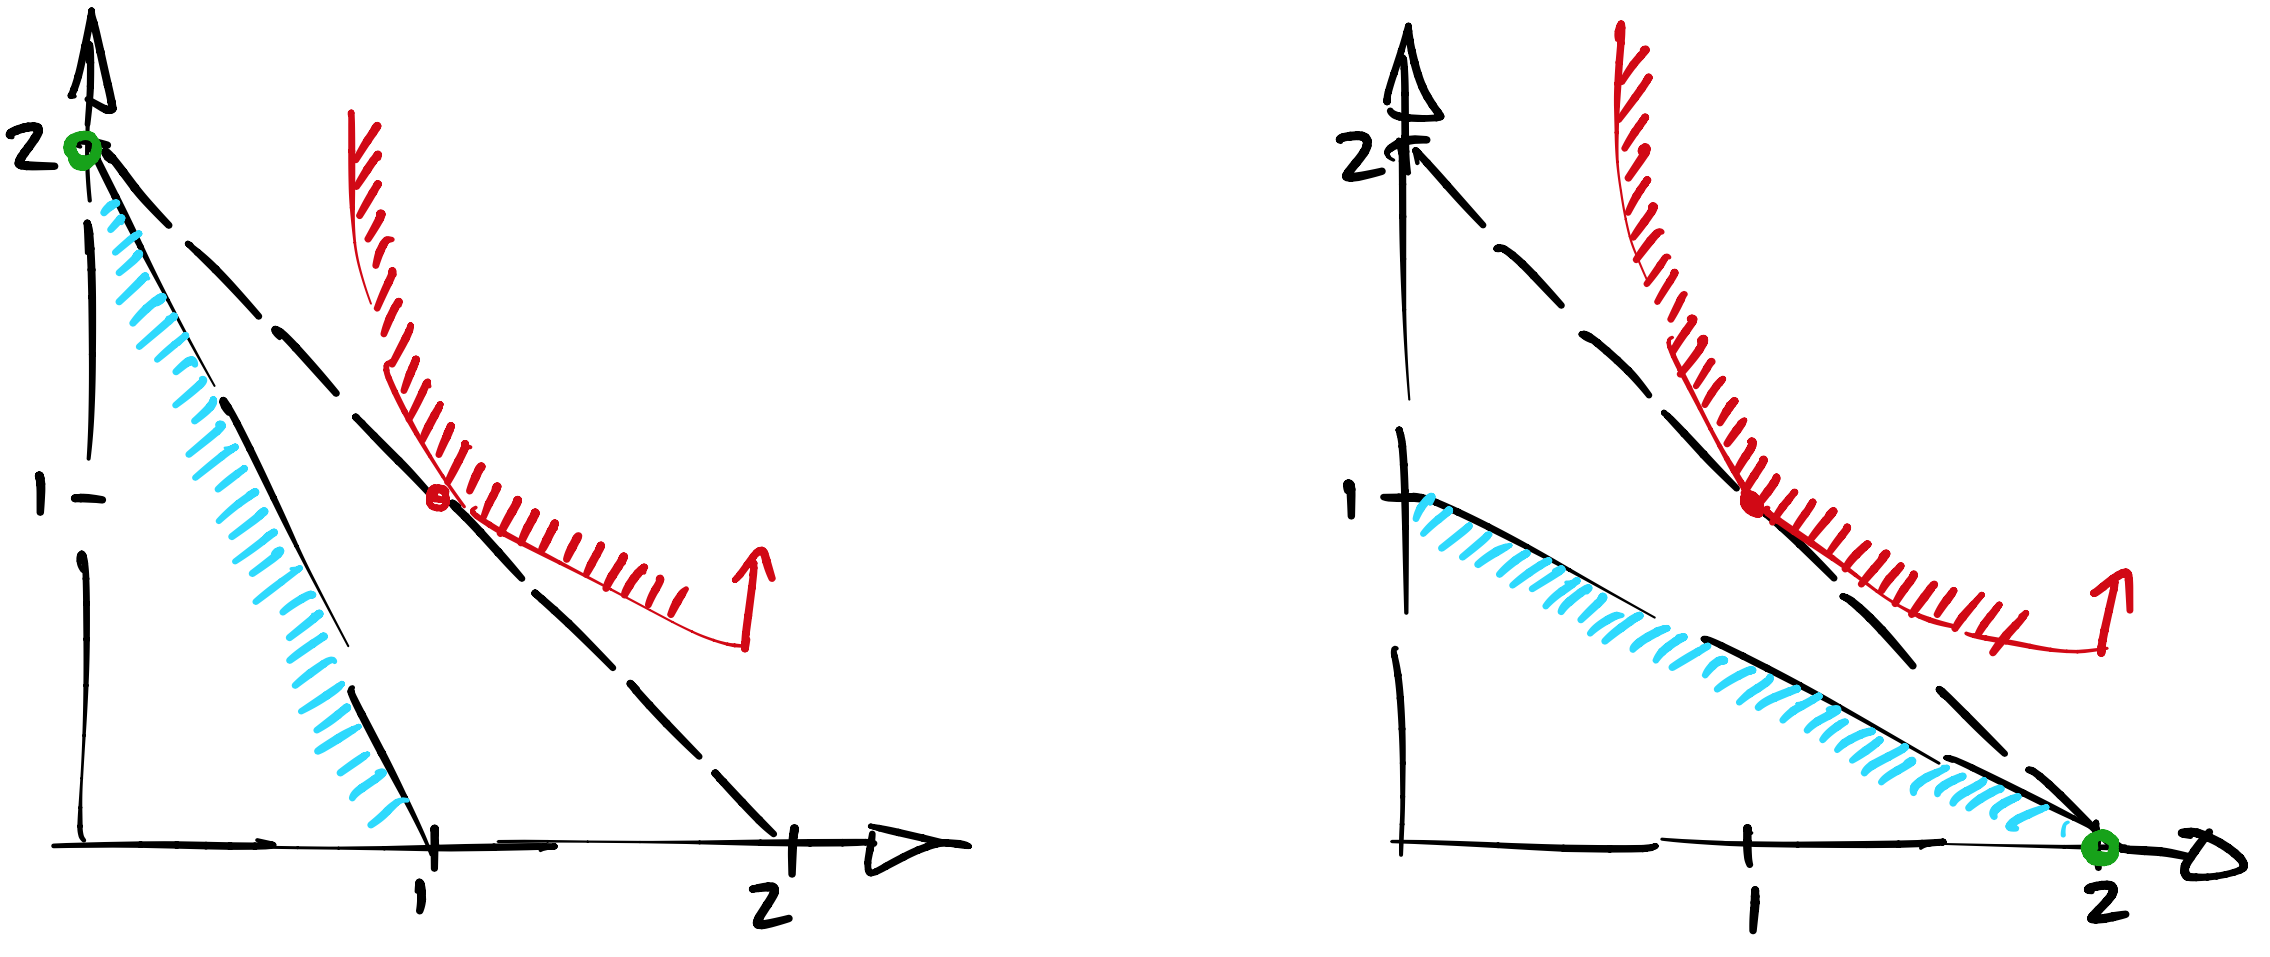
\includegraphics[width=1 \textwidth]{pic2.png}
\end{figure}
Выведем их на доске.
\end{frame}

\begin{frame}{Пример 1}
Подведем итог.

\begin{itemize}
  \item Первая страна специализируется на производстве товара $y$
  \item Вторая страна специализируется на производстве товара $x$
  \item Экспорт товара $x$ идет из второй страны в первую
  \item Каждый агент выберет точку, недоступную в автаркии
  \item Каждый агент повысит свою полезность на $$\log (1) - \log (1/2) > 0$$
  \end{itemize}

\end{frame}

\section{Пример 2}

\begin{frame}{Пример 1}

В предыдущем примере выгода от торговли была очевидна. А что если одна из двух стран обладает абсолютным преимуществом в производстве всех товаров.
$$ F_1(X,Y) = X + Y/2 - 1 \leqslant 0, \quad F_2(X,Y) = X/4 + Y/2 - 1 \leqslant 0$$

Будет ли торговля оптимальной тогда?

\end{frame}

\begin{frame}{Пример 2}

Пусть цена товара $x$ нормирована к 1, а цена товара $y$ равна $q$.

Найдем равновесие в автаркии

УПП для первой страны можно записать как
$$ \frac{1/x}{1/y} = \frac{1}{1/2} = \frac{1}{q} \quad \Rightarrow \quad q = 1/2, \ y = 2x$$
Подставляя в соответствующие технологические границы, мы получаем координаты потребления $(1/2,1)$ для первой страны и полезность $\log(1/2) + \log(1)$.

\end{frame}

\begin{frame}{Пример 2}

УПП для второй страны можно записать как
$$ \frac{1/x}{1/y} = \frac{1/4}{1/2} = \frac{1}{q} \quad \Rightarrow \quad q = 2, \ y = x/2$$
Подставляя в соответствующие технологические границы, мы получаем координаты потребления $(1/2,1/4)$ для второй страны и полезность $\log(1/2) + \log(1/4)$.

\end{frame}

\begin{frame}{Пример 2}

Так же как и в первом примере, поскольку цена товара $y$ выше во второй стране, то при международной торговле товар $y$ будет экспортироваться в направлении второй страны, а $x$, наоборот, в направлении первой страны. Цены будут двигаться навстречу друг другу до тех пор, пока не встретятся где-то посередине.

Совместное технологическое множество это такая *трапеция* с изломом в точке $(4,2)$.

\end{frame}

\begin{frame}{Пример 2}

Напомню, что мы используем трюк с гомотетичностью
\begin{figure}[hbt]
\centering
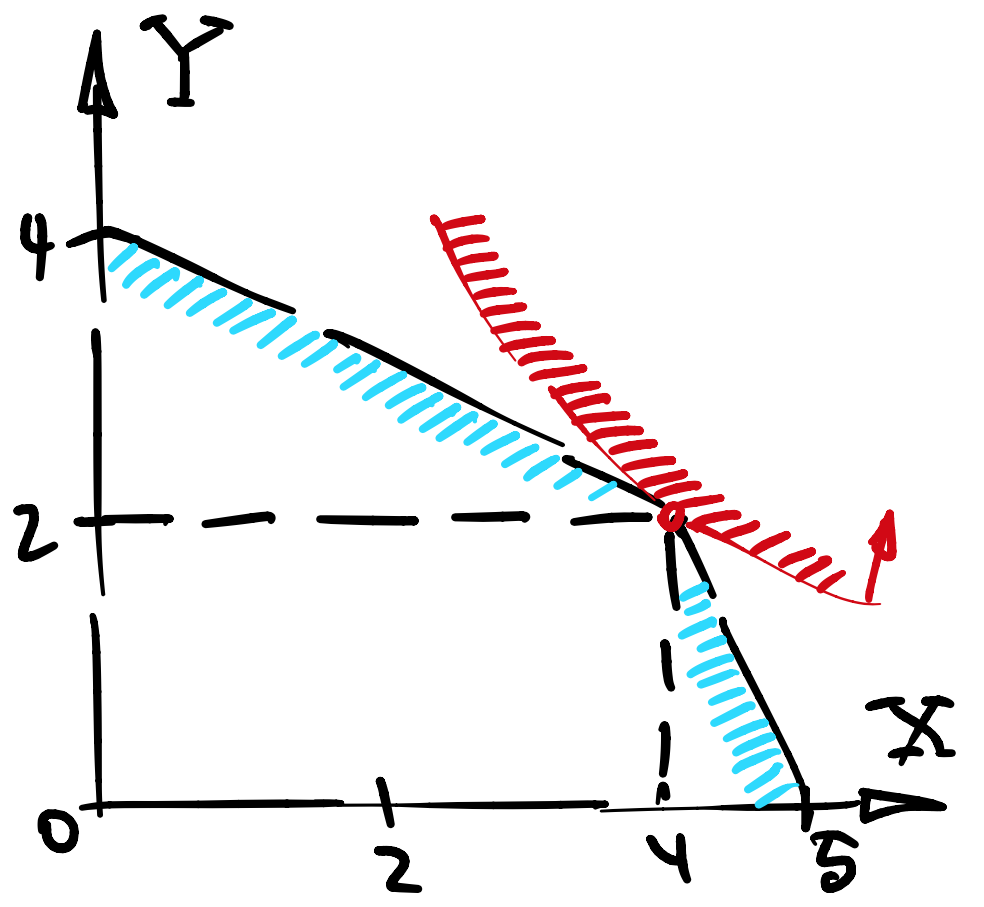
\includegraphics[width=.6 \textwidth]{pic3.png}
\end{figure}
\end{frame}

\begin{frame}{Пример 2}

Всего возможно три варианта, в котором будет равновесие:

\begin{itemize}
  \item если производство на верхней арке технологического множества, тогда цена будет как во второй стране, то есть, $q = 2$
  \item если производство на правой арке технологического множества, тогда цена будет как в первой стране, то есть, $q = 1/2$
  \item если производство на изломе, тогда цены неизвестны, но известно что одна страна производит $4$ единицы товара $x$ а другая 2 единицы товара $y$
\end{itemize}
Вообще, \alert{равновесная цена всегда должна находиться в интервале между ценами автаркии}.

\end{frame}

\begin{frame}{Пример 2}
Дорешаем у доски. В оставшееся время

\begin{itemize}
  \item Леонтьевская полезность
  \item Гладкие КПВ
  \item Разные полезности
\end{itemize}
\end{frame}

\end{document}
